\section{Defining Problem}
In the Maze problem, our goal is to 
start from a point and reach some goal 
point bypassing obstacles through the way. 
To represent the maze map, we are using a grid map. 
Grid maps represent every point that agents can be by 
a square with some specific color and obstacles with 
another color.
\begin{figure}[H]
    \centering
  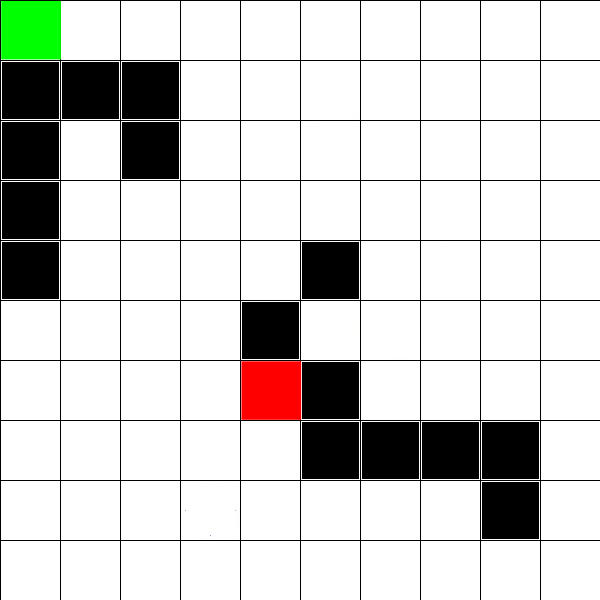
\includegraphics[width = .5\textwidth ]{images/map.png}
  \caption{example of a grid map that agent need to start from green
            square and reach red one. black squares represent obstacles.}
  \label{fig:gird-map}
\end{figure}